This section presents our work with a demographic filter for recommending top trending movies.
That is, "best" movies in the entire dataset are presented as such.\\
The challenge, precisely, is defining how to say that certain movies are the best.

\subsection*{Metric}
We choose the \emph{weighted average rating}
\footnote{\href{https://math.stackexchange.com/questions/169032/understanding-the-imdb-weighted-rating-function-for-usage-on-my-own-website}{https://math.stackexchange.com/questions/169032/understanding-the-imdb-weighted-rating-function-for-usage-on-my-own-website}}
for assigning a value to each of the movies in our dataset, the same used by \href{https://www.imdb.com/chart/top?ref_=nb\_mv\_3\_chttp}{IMDb}.
\begin{center}
    \(WAR = \left(\frac{v}{v+m} \cdot R\right) + \left(\frac{m}{v+m} \cdot C\right)\)
\end{center}
Being:
\begin{itemize}
    \item v $\Rightarrow$ number of votes for the movie
    \item m $\Rightarrow$ minimum votes required to be listed
    \item R $\Rightarrow$ average rating of the movie
    \item C $\Rightarrow$ mean vote for every movie
\end{itemize}

\subsection*{Implementation}
Implementing this recommender means assigning the described score to each movie entry in the dataset,
then sort them descending by their weighted average score,
and finally take the top 10 movies. They are the 10 trending movies.
\begin{center}
    \captionsetup{type=figure}
    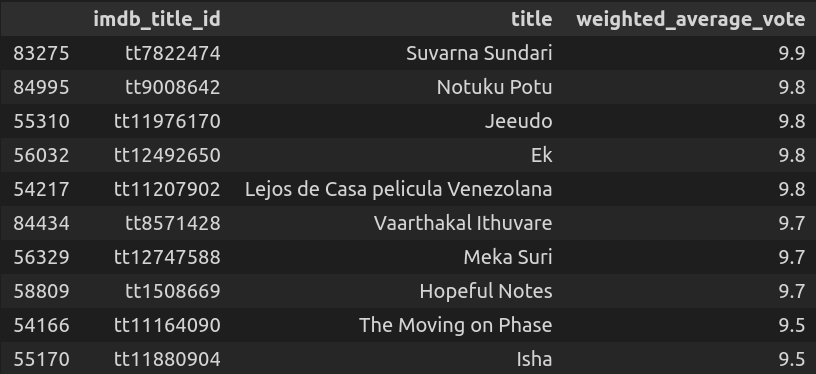
\includegraphics[width=250px]{images/demo-result.png}
    \captionof{figure}{Demographic Filtering Result}
\end{center} 
%TODO: caching?
